\chapter{L-Systems}

\section{¿Qué son los L-Systems?}

\noindent Un sistema-L o también denominados sistemas de Lindenmayer se trata de un conjunto de reglas y símbolos usados principalmente para modelar el proceso de crecimiento de las plantas.

\noindent Fueron introducidos en 1968 por Aristid Lindenmayer, el cual estudió los patrones de crecimiento de varias algas y tenían como objetivo realizar una descripción formal del desarrollo de organismos y representar la relación entre células de plantas.

\section{¿Cómo funcionan?}

\noindent Las reglas de estos sistemas se basa en la autosimilitud, por eso las figuras que se suelen modelar suelen representar formas de tipo fractal.

\noindent Los sistemas-L se definen como un conjunto $G=\{V,S, \omega ,P\}$

\begin{itemize}
    \item $V$ es un conjunto de símbolos que contiene elementos que pueden ser reemplazados.
    \item $S$ es un conjunto de símbolos que contiene elementos que se mantienen fijos.
    \item $\omega$ es una cadena de símbolos de $V$ que definen el estado inicial del sistema (inicio o axioma).
    \item $P$ es un conjunto de reglas o producciones que definen la forma en la que las variables pueden ser reemplazadas por combinaciones de constantes y otras variables.
\end{itemize}

\noindent Todos los sistemas-L parten de un estado inicial, y se dice que el sistema es libre de contexto si cada iteración se refiere sólo a un símbolo individual y no a sus vecinos. Cuando la aplicación de una regla depende también de sus vecinos, se dice que el sistema-L es sensitivo al contexto.

\section{Ejemplos}

\subsection{Algas}

\noindent Pongamos como ejemplo de sistema-L el primer caso que quiso estudiar Lindenmayer, las algas.

\noindent Datos:

\begin{itemize}
    \item Variables: $A,B$
    \item Constantes: ninguna
    \item Incio: $A$
    \item Reglas: $A \rightarrow AB, B \rightarrow A$
\end{itemize}

\noindent Resultado:

\begin{itemize}
    \item Iteración 0: $A$
    \item Iteración 1: $AB$
    \item Iteración 2: $ABA$
    \item Iteración 3: $ABAAB$
    \item Iteración 4: $ABAABABA$
    \item Iteración 5: $ABAABABAABAAB$
\end{itemize}

\subsection{Copos de nieve}

\noindent Los sistemas también pueden ser representado con dibujos, el siguiente ejemplo se refiere a la variante de la curva de Koch con ángulo de 90:\\

\noindent Sintaxis:

\begin{equation}
    \begin{split}
        & F\rightarrow \text{Dibujar hacia adelante}\\
        & +\rightarrow \text{Girar a la izquierda } 90 \text{ grados}\\
        & -\rightarrow \text{Girar a la derecha } 90 \text{ grados}\\
    \end{split}
\end{equation}

\noindent Datos:

\begin{itemize}
    \item Variables: $F$
    \item Constantes: $+,-$
    \item Incio: $F$
    \item Reglas: $F \rightarrow F+F-F-F+F$
\end{itemize}

\noindent Resultado:\\

\noindent Para $n=0$ tenemos $F$:

\begin{figure}[H]
    
    \centering
    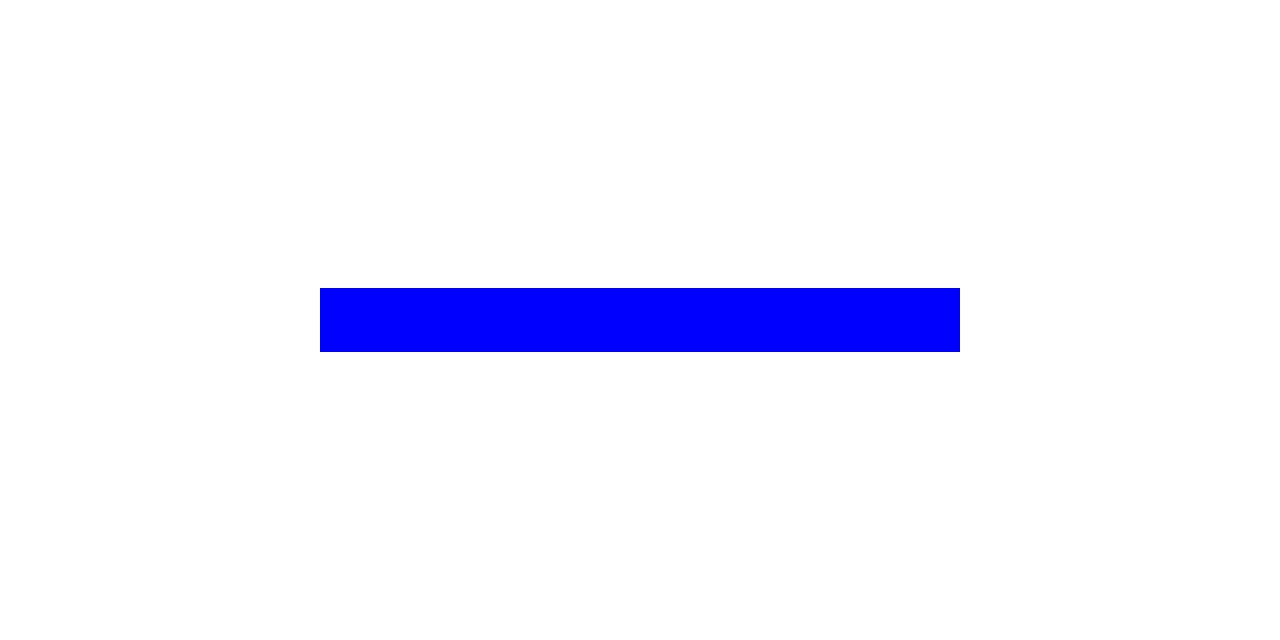
\includegraphics[width=0.5\textwidth]{figures/l-system-kock-snowflake-1.png}
    \caption{Curva de Koch con ángulo de 90 grados - 0 iteraciones}
    \label{fig:koch-snowflake-1}
\end{figure}

\noindent Para $n=1$ tenemos $F+F-F-F+F$:

\begin{figure}[H]
    \centering
    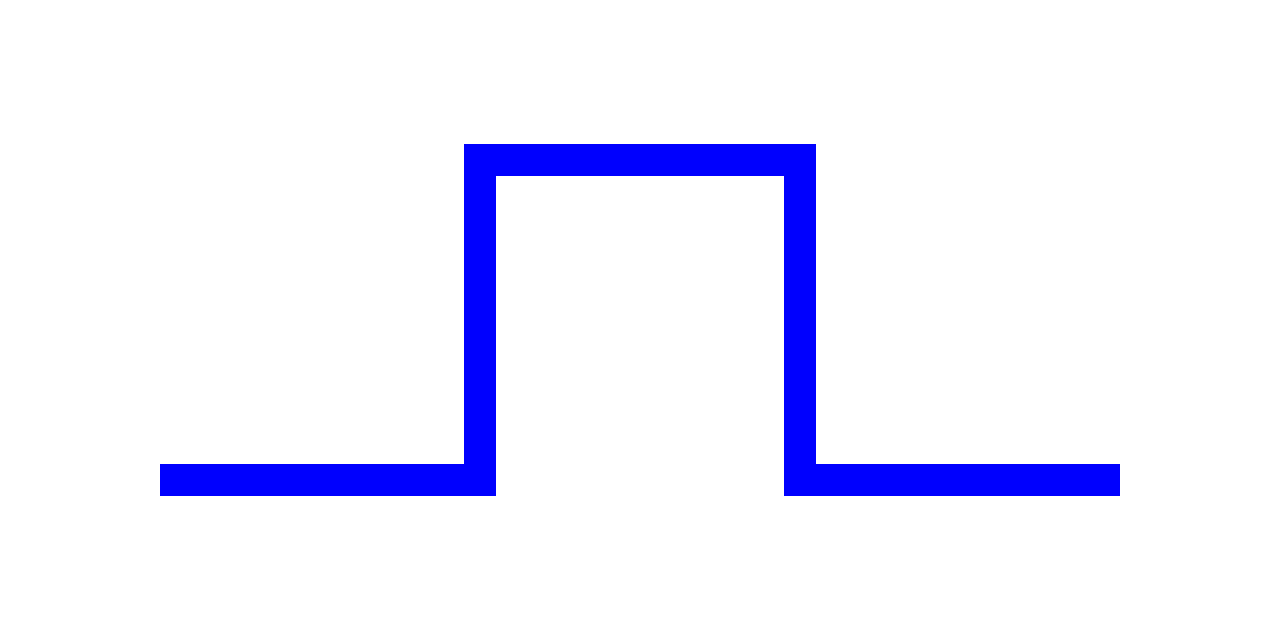
\includegraphics[width=0.5\textwidth]{figures/l-system-kock-snowflake-2.png}
    \caption{Curva de Koch con ángulo de 90 grados - 1 iteración}
    \label{fig:koch-snowflake-2}
\end{figure}

\noindent Para $n=2$ tenemos $F+F-F-F+F+F+F-F-F+F-F+F-F-F+F-F+F-F-F+F+F+F-F-F+F$:

\begin{figure}[H]
    \centering
    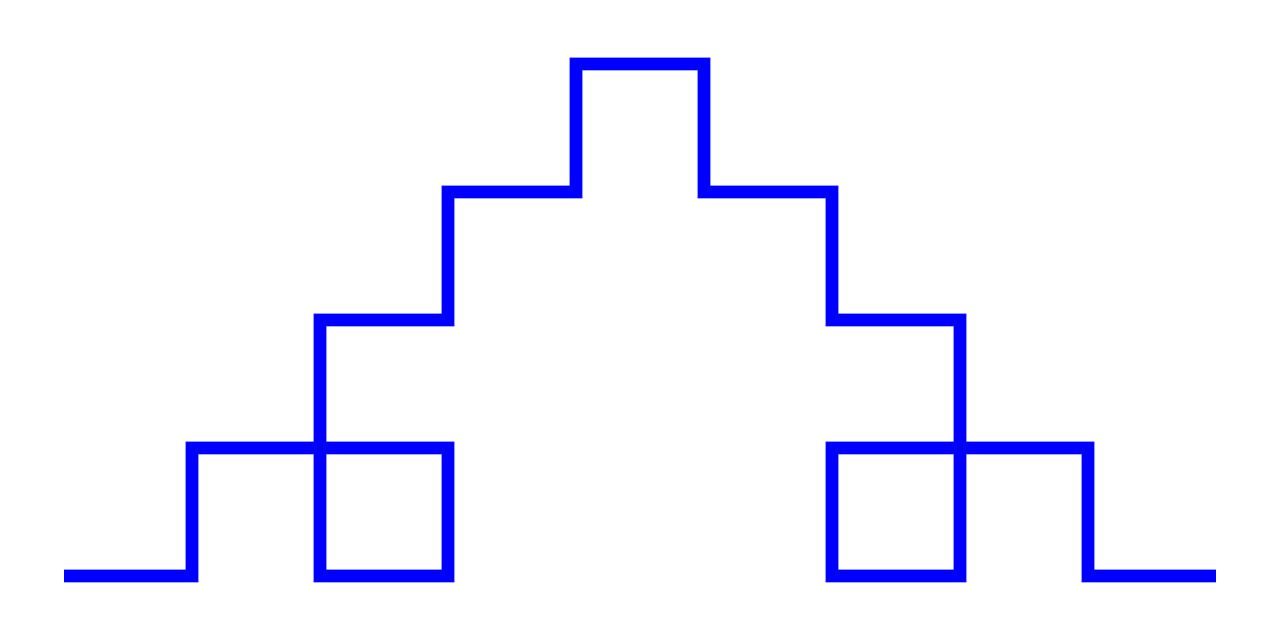
\includegraphics[width=0.5\textwidth]{figures/l-system-kock-snowflake-3.png}
    \caption{Curva de Koch con ángulo de 90 grados - 2 iteraciones}
    \label{fig:koch-snowflake-3}
\end{figure}

\noindent Para $n=3$ la secuencia es demasiado larga para ponerla aquí, pero el resultado es el siguiente:

\begin{figure}[H]
    \centering
    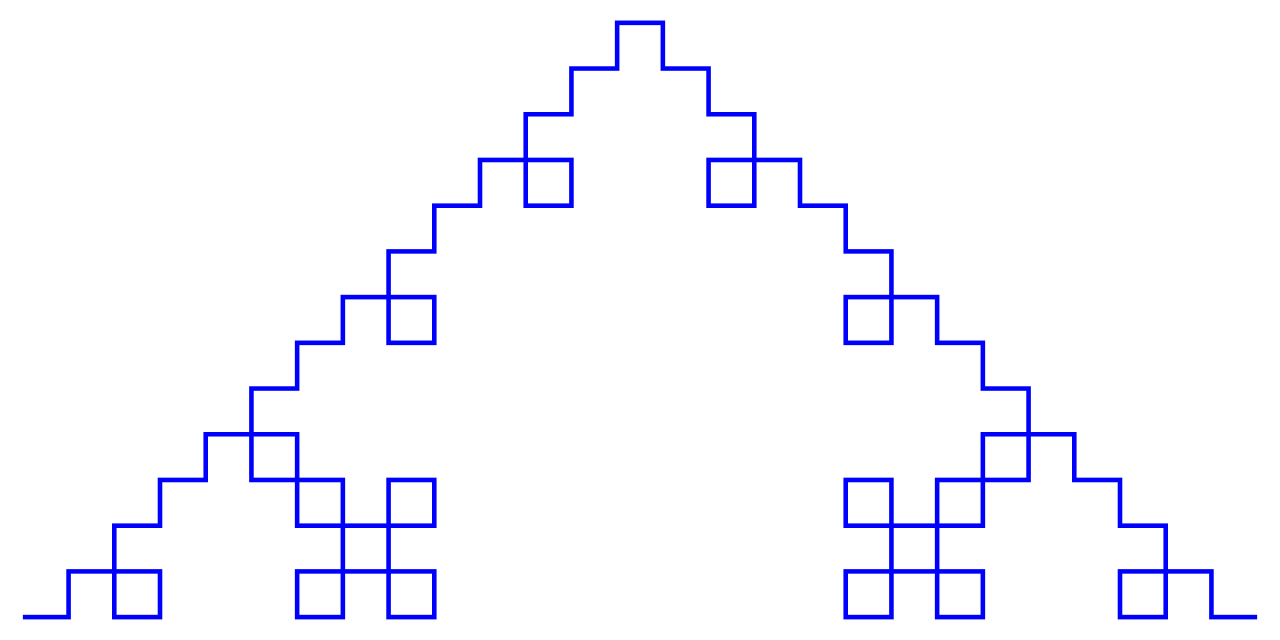
\includegraphics[width=0.5\textwidth]{figures/l-system-kock-snowflake-4.png}
    \caption{Curva de Koch con ángulo de 90 grados - 3 iteraciones}
    \label{fig:koch-snowflake-4}
\end{figure}

\section{Dibujos de plantas con L-Systems}

\subsection{Planta 1}

\begin{figure}[H]
    \centering
    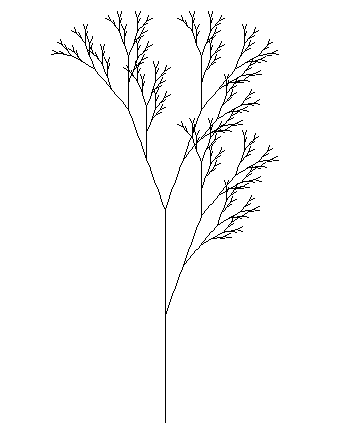
\includegraphics[width=0.5\textwidth]{figures/l-system-plant-1.png}
    \caption{Planta 1}
    \label{fig:plant-1}
    \cite{web-2023}
\end{figure}

\subsection{Planta 2}

\begin{figure}[H]
    \centering
    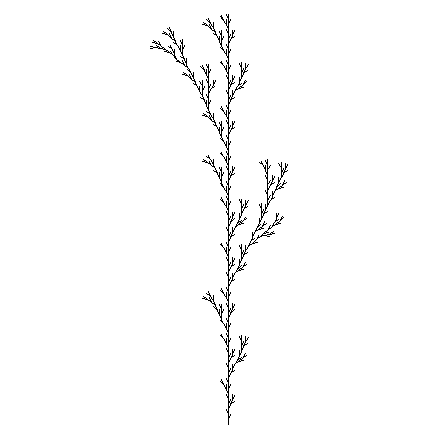
\includegraphics[width=0.5\textwidth]{figures/l-system-plant-2.png}
    \caption{Planta 2}
    \label{fig:plant-2}
    \cite{web-2023}
\end{figure}

\subsection{Planta 3}

\begin{figure}[H]
    \centering
    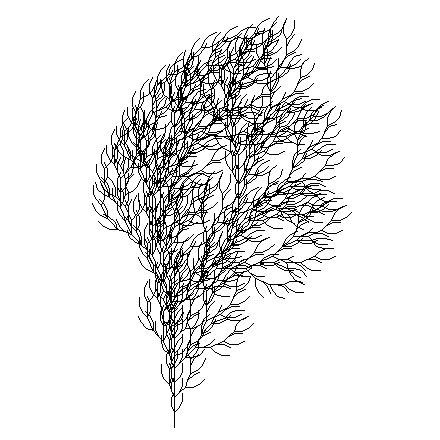
\includegraphics[width=0.5\textwidth]{figures/l-system-plant-3.png}
    \caption{Planta 3}
    \label{fig:plant-3}
    \cite{web-2023}
\end{figure}